\documentclass[]{article}

\def\nno{\nonumber}
\def\bfE{\mbox{\boldmath$E$}}
\def\bfG{\mbox{\boldmath$G$}}
\def \p{\partial}
\usepackage{epsfig, color}
\usepackage{color,graphicx}
\usepackage{amsfonts}
\usepackage{color}
\usepackage{amsmath}
\usepackage{amssymb}
\usepackage{amsthm}
\usepackage{natbib}
\usepackage{fancybox}
\usepackage{ulem}
\usepackage{subfigure}
\usepackage{multirow}
\usepackage{bbm}
\usepackage{enumerate}
\usepackage{rotating}
\usepackage{float}
\usepackage{epstopdf}
\usepackage{tcolorbox}
\usepackage{mdframed}
\usepackage{framed}
\usepackage{graphbox}
\usepackage{makecell}
\usepackage{diagbox}
\usepackage{booktabs}
\usepackage{threeparttable}
\usepackage{appendix}

%\usepackage{refcheck}

\allowdisplaybreaks[4]

\newtheorem{definition}{\hspace{6mm}Definition}[section]
\newtheorem{theorem}{\hspace{6mm}Theorem}[section]
%\newtheorem{lemma}{\hspace{6mm}Lemma}[section]
\newtheorem{remark}{\hspace{6mm}Remark}[section]
\newtheorem{lemma}[theorem]{\hspace{6mm}Lemma}
%\newtheorem{remark}[theorem]{Remark}
\newtheorem{example}{\textsc{Example}}[section]
\newtheorem{proposition}{\hspace{6mm}Proposition}[section]
\newtheorem{algorithm}{Algorithm}
\renewcommand{\(}{\left(}
\renewcommand{\)}{\right)}
\newcommand{\bm}[1]{\mbox{\boldmath{$#1$}}}
\def\cred{\color{red}}
\def\cblue{\color{blue}}
\def\cgreen{\color{green}}

%opening
\title{Deep signature transforms for rough volatility model}
\author{}
\date{}

\begin{document}
	
	\maketitle
	
	%\begin{abstract}
	%
	%\end{abstract}
	
	\section{Preliminary numerical experiments}
	\subsection{Implementation details}\label{sec1}
	In the following numerical experiments, we will introduce various neural network models to calibrate parameters from time series data generated by fractional Brownian motions and rough Bergomi volatility processes.
	\subsubsection{Models' architecture}
	We first clarify the architecture of these neural network models that we will use in the following numerical experiments.
	
	The DeepSigNet model is a neural network model with signature transform proposed by \cite{Lyons_2019_DeepSignature}. The CNN model is a convolutional neural network proposed by \cite{stone_2020}. And we also provide another maxpooling CNN model and signature CNN model to explore whether the signature transform is a better choice than the maxpooling layer. The specific structures of these models are presented below:
	\begin{itemize}
		\item The DeepSigNet model:
		\begin{itemize}
			\item[-]a convolutional layer with 3 channels and kernel size 3;
			\item[-]augmented with time and original values;
			\item[-]the signature transform with truncation order $N=3$;
			\item[-]a fully connected feedforward neural network with 5 hidden layers, each of size 32 and ReLU activation;
			\item[-]the non-linear transform with sigmoid function.
		\end{itemize}
		\item The CNN model:
		\begin{itemize}
			\item[-]a convolutional layer with 32 channels and kernel size 20;
			\item[-]the leaky ReLu transform with negative slope 0.1;
			\item[-]a max pooling layer with size 3;
			\item[-]a dropout layer with rate 0.25;			
			\item[-]a convolutional layer with 64 channels and kernel size 20;
			\item[-]the leaky ReLu transform with negative slope 0.3;
			\item[-]a max pooling layer with size 3;
			\item[-]a dropout layer with rate 0.25;
			\item[-]a convolutional layer with 128 channels and kernel size 20;
			\item[-]the leaky ReLu transform with negative slope 0.1;
			\item[-]a max pooling layer with size 3;
			\item[-]a dropout layer with rate 0.4;
			\item[-]a dense layer with 128 units;
			\item[-]the leaky ReLu transform with negative slope 0.1;
			\item[-]a dropout layer with rate 0.3;
			\item[-]a dense layer with 1 units;
			\item[-]the non-linear transform with sigmoid function.			
		\end{itemize}
		\item The maxpooling CNN model:
		\begin{itemize}
			\item[-]a convolutional layer with 32 channels and kernel size 20;
			\item[-]the leaky ReLu transform with negative slope 0.1;
			\item[-]a max pooling layer with size 3;
			\item[-]a dropout layer with rate 0.25;
			\item[-]a dense layer with 128 units;
			\item[-]the leaky ReLu transform with negative slope 0.1;
			\item[-]a dropout layer with rate 0.25;
			\item[-]a dense layer with 1 units;	
			\item[-]the non-linear transform with sigmoid function.
		\end{itemize}
		\item The signature CNN model:
		\begin{itemize}
			\item[-]a convolutional layer with 32 channels and kernel size 20;
			\item[-]the leaky ReLu transform with negative slope 0.1;
			\item[-]the signature transform with truncation order $N=2$;
			\item[-]a dropout layer with rate 0.25;
			\item[-]a dense layer with 128 units;
			\item[-]the leaky ReLu transform with negative slope 0.1;
			\item[-]a dropout layer with rate 0.25;
			\item[-]a dense layer with 1 units;
			\item[-]the non-linear transform with sigmoid function.	
		\end{itemize}
	\end{itemize}
	\subsubsection{Simulated data set}
	We use simulated sample paths of fractional Brownian motions (fBm) $\{Z_t\}$ and rough Bergomi (rBergomi) volatility processes $\{V_t\}$ as the input data. 
	The fractional Brownian motion is defined as 
	\begin{equation}
		Z_t = \int_{0}^{t} (t-s)^{H-\frac{1}{2}} dW_s,\quad t>0,
	\end{equation}
	where $H\in(0,1)$ is the Hurst parameter and $W$ is a standard Brownian motion.
	The rBergomi volatility process is defined as
	\begin{equation}
		V_t = V_0 \exp \left(\eta\sqrt{2H}Z_t - \frac{\eta^2}{2} t^{2H}\right),\quad V_0>0,
	\end{equation}
	where $\eta$ is a strictly positive constant.
	
	To simulate these sample paths we use Cholesky decomposition; this very well-known simulation technique is recommended because the resulting sample paths have the exact distribution, rather than an approximate distribution, of the normalised log volatility process of the rBergomi model.

	\subsection{Supervised learning with fractional Brownian motion and rough Bergomi volatility process}
	In this example, we first let the Hurst parameter $H$ takes values in the discrete grid $\{0.1, 0.2, 0.3, 0.4, 0.5\}$ and we also sample $5$ $H$ values from different probability distributions: the Uniform distribution\footnote{The corresponding set of possible $H$ values is $\{0.05, 0.18, 0.29, 0.31, 0.44\}$.} on $(0,0.5)$ and the $\text{Beta}(1, 9)$ distribution\footnote{The corresponding set of possible $H$ values is $\{0.02, 0.06, 0.07, 0.13, 0.22\}$.}. Then we use these different $H$ to simulate fBm and rBergomi paths ($\eta=1$) with different number of time steps $\{100,200,300,400,500\}$ to generate five corresponding training/test data sets and the sizes of each data set are given in Table~\ref{tab-H-datasize}. 
	\begin{table}[H]
		\caption{Training and test data size.}
		\label{tab-H-datasize}
		\smallskip
		\centering
		\renewcommand\arraystretch{1.5}
		\begin{tabular}{l c}
			\toprule
			Data set&Number of samples\\
			\hline
			Training set&2800\\
			Test set&700\\	
			\bottomrule
		\end{tabular}
	\end{table}
	We use adaptive moment estimation (Adam) to train the networks with the architecture\footnote{The code for DeepSigNet model is provided by the original paper and My DeepSigNet model has the same structure with DeepSigNet but recoded by myself with Pytorch. The CNN is also recoded by Pytorch with the same structure as the original paper.} described in Section~\ref{sec1}, setting $batch\, size=64$, $epochs=100$ as is fairly standard. We use the mean square error (MSE) as the loss function for training and we also provide the root mean square error (RMSE) in test results as reference. The test results are shown in Table~\ref{tab-discrete-H}-\ref{tab-beta-H} and the loss plots are shown in Appendix~\ref{appendix-loss-plot}.
	
	There are some remarks for the results below:
	\begin{itemize}
		\item The number of parameters in DeepSigNet remains stable regardless of the input length, indicating that the model's complexity remains stable across different input lengths.
		\item My DeepSigNet slightly outperforms DeepSigNet in most cases. But both of them outperform than CNN including the results in \cite{stone_2020}.
		\item The Maxpooling CNN slightly outperforms Signature CNN but significantly underperforms DeepSigNet. This may due to the fact that the first convolutional layer of Signature CNN significantly increases the number of sequence features used for signature transform.
	\end{itemize}
	\begin{table}[H]
		\caption{Test results for discretised $H$.}
		\label{tab-discrete-H}
		\smallskip
		\centering
		\renewcommand\arraystretch{1.5}
		\resizebox{0.9\textwidth}{!}{\begin{tabular}{l c c c c c c}
				\toprule
				\multirow{2}{*}{Models}&\multirow{2}{*}{Input length}&\multicolumn{2}{c}{fBm}&\multicolumn{2}{c}{rBergomi}&\multirow{2}{*}{$\#$Params}\\
				\cline{3-4}\cline{5-6}
				&&MSE&RMSE&MSE&RMSE&\\
				\hline
				\multirow{5}{*}{DeepSigNet}&100&$1.18\times10^{-4}$&$1.08\times10^{-2}$&$8.87\times10^{-4}$&$2.84\times10^{-2}$&9261\\
				&200&$3.00\times10^{-5}$&$5.36\times10^{-3}$&$4.51\times10^{-4}$&$2.10\times10^{-2}$&9261\\
				&300&$3.63\times10^{-5}$&$5.94\times10^{-3}$&$2.43\times10^{-4}$&$1.54\times10^{-2}$&9261\\
				&400&$4.48\times10^{-5}$&$6.61\times10^{-3}$&$1.85\times10^{-4}$&$1.33\times10^{-2}$&9261\\
				&500&$3.75\times10^{-5}$&$6.02\times10^{-3}$&$2.14\times10^{-4}$&$1.45\times10^{-2}$&9261\\
				\hline
				\multirow{5}{*}{My DeepSigNet}&100&$1.09\times10^{-5}$&$2.05\times10^{-3}$&$4.96\times10^{-4}$&$2.22\times10^{-2}$&9261\\
				&200&$2.59\times10^{-6}$&$1.55\times10^{-3}$&$2.48\times10^{-4}$&$1.56\times10^{-2}$&9261\\
				&300&$1.38\times10^{-5}$&$3.67\times10^{-3}$&$2.33\times10^{-4}$&$1.52\times10^{-2}$&9261\\
				&400&$2.55\times10^{-6}$&$1.49\times10^{-3}$&$1.95\times10^{-4}$&$1.38\times10^{-2}$&9261\\
				&500&$6.88\times10^{-6}$&$2.34\times10^{-3}$&$1.18\times10^{-4}$&$1.07\times10^{-2}$&9261\\
				\hline
				\multirow{5}{*}{CNN}&100&$2.11\times10^{-3}$&$4.59\times10^{-2}$&$2.51\times10^{-3}$&$4.97\times10^{-2}$&255073\\
				&200&$2.21\times10^{-3}$&$4.69\times10^{-2}$&$1.57\times10^{-3}$&$3.96\times10^{-2}$&320609\\
				&300&$2.66\times10^{-3}$&$5.16\times10^{-2}$&$2.16\times10^{-3}$&$4.62\times10^{-2}$&386145\\
				&400&$2.44\times10^{-3}$&$4.93\times10^{-2}$&$1.51\times10^{-3}$&$3.88\times10^{-2}$&435297\\
				&500&$1.84\times10^{-3}$&$4.29\times10^{-2}$&$1.88\times10^{-3}$&$4.32\times10^{-2}$&500833\\
				\hline
				\multirow{5}{*}{Maxpooling CNN}&100&$1.90\times10^{-3}$&$4.36\times10^{-2}$&$1.70\times10^{-3}$&$4.11\times10^{-2}$&136097\\
				&200&$2.00\times10^{-3}$&$4.46\times10^{-2}$&$1.28\times10^{-3}$&$3.57\times10^{-2}$&271265\\
				&300&$2.49\times10^{-3}$&$4.98\times10^{-2}$&$1.81\times10^{-3}$&$4.24\times10^{-2}$&410529\\
				&400&$2.01\times10^{-3}$&$4.47\times10^{-2}$&$1.27\times10^{-3}$&$3.56\times10^{-2}$&545697\\
				&500&$1.29\times10^{-3}$&$3.58\times10^{-2}$&$1.38\times10^{-3}$&$3.70\times10^{-2}$&680865\\
				\hline
				\multirow{5}{*}{Signature CNN}&100&$2.51\times10^{-3}$&$5.00\times10^{-2}$&$3.40\times10^{-3}$&$5.81\times10^{-2}$&136097\\
				&200&$2.46\times10^{-3}$&$4.95\times10^{-2}$&$3.95\times10^{-3}$&$6.28\times10^{-2}$&136097\\
				&300&$2.07\times10^{-3}$&$4.54\times10^{-2}$&$2.96\times10^{-3}$&$5.42\times10^{-2}$&136097\\
				&400&$3.26\times10^{-3}$&$5.70\times10^{-2}$&$2.97\times10^{-3}$&$5.43\times10^{-2}$&136097\\
				&500&$2.56\times10^{-3}$&$5.05\times10^{-2}$&$2.96\times10^{-3}$&$5.41\times10^{-2}$&136097\\
				\bottomrule
		\end{tabular}}
	\end{table}
	
	\begin{table}[H]
		\caption{Test results for $H\sim\text{Uniform}(0,0.5)$.}
		\label{tab-uniform-H}
		\smallskip
		\centering
		\renewcommand\arraystretch{1.5}
		\resizebox{0.9\textwidth}{!}{\begin{tabular}{l c c c c c c}
				\toprule
				\multirow{2}{*}{Models}&\multirow{2}{*}{Input length}&\multicolumn{2}{c}{fBm}&\multicolumn{2}{c}{rBergomi}&\multirow{2}{*}{$\#$Params}\\
				\cline{3-4}\cline{5-6}
				&&MSE&RMSE&MSE&RMSE&\\
				\hline
				\multirow{5}{*}{DeepSigNet}&100&$8.22\times10^{-5}$&$9.00\times10^{-3}$&$1.25\times10^{-3}$&$3.52\times10^{-2}$&9261\\
				&200&$1.61\times10^{-4}$&$1.25\times10^{-2}$&$3.18\times10^{-4}$&$1.75\times10^{-2}$&9261\\
				&300&$5.58\times10^{-4}$&$2.35\times10^{-2}$&$4.94\times10^{-4}$&$2.21\times10^{-2}$&9261\\
				&400&$5.56\times10^{-4}$&$2.35\times10^{-2}$&$2.05\times10^{-4}$&$1.42\times10^{-2}$&9261\\
				&500&$5.14\times10^{-4}$&$2.25\times10^{-2}$&$1.07\times10^{-3}$&$2.23\times10^{-2}$&9261\\
				\hline
				\multirow{5}{*}{My DeepSigNet}&100&$3.07\times10^{-5}$&$5.48\times10^{-3}$&$8.47\times10^{-4}$&$2.89\times10^{-2}$&9261\\
				&200&$1.95\times10^{-5}$&$4.39\times10^{-3}$&$2.13\times10^{-4}$&$1.44\times10^{-2}$&9261\\
				&300&$4.26\times10^{-5}$&$6.40\times10^{-3}$&$4.91\times10^{-4}$&$2.19\times10^{-2}$&9261\\
				&400&$1.65\times10^{-5}$&$4.04\times10^{-3}$&$1.25\times10^{-4}$&$1.11\times10^{-2}$&9261\\
				&500&$7.78\times10^{-5}$&$8.48\times10^{-3}$&$4.36\times10^{-4}$&$1.59\times10^{-2}$&9261\\
				\hline
				\multirow{5}{*}{CNN}&100&$1.90\times10^{-3}$&$4.35\times10^{-2}$&$2.83\times10^{-3}$&$5.31\times10^{-2}$&255073\\
				&200&$1.81\times10^{-3}$&$4.25\times10^{-2}$&$1.66\times10^{-3}$&$4.06\times10^{-2}$&320609\\
				&300&$1.62\times10^{-3}$&$4.02\times10^{-2}$&$2.15\times10^{-3}$&$4.63\times10^{-2}$&386145\\
				&400&$1.23\times10^{-2}$&$1.10\times10^{-1}$&$2.45\times10^{-3}$&$4.94\times10^{-2}$&435297\\
				&500&$1.96\times10^{-3}$&$4.42\times10^{-2}$&$1.64\times10^{-3}$&$4.05\times10^{-2}$&500833\\
				\hline
				\multirow{5}{*}{Maxpooling CNN}&100&$1.10\times10^{-3}$&$3.31\times10^{-2}$&$2.74\times10^{-3}$&$5.23\times10^{-2}$&136097\\
				&200&$1.35\times10^{-3}$&$3.67\times10^{-2}$&$1.60\times10^{-3}$&$3.99\times10^{-2}$&271265\\
				&300&$1.20\times10^{-3}$&$3.46\times10^{-2}$&$1.50\times10^{-3}$&$3.86\times10^{-2}$&410529\\
				&400&$8.62\times10^{-4}$&$2.93\times10^{-2}$&$1.50\times10^{-3}$&$3.85\times10^{-2}$&545697\\
				&500&$5.94\times10^{-4}$&$2.42\times10^{-2}$&$1.36\times10^{-3}$&$3.67\times10^{-2}$&680865\\
				\hline
				\multirow{5}{*}{Signature CNN}&100&$1.72\times10^{-3}$&$4.14\times10^{-2}$&$2.83\times10^{-3}$&$5.30\times10^{-2}$&136097\\
				&200&$1.69\times10^{-3}$&$4.10\times10^{-2}$&$2.89\times10^{-3}$&$5.36\times10^{-2}$&136097\\
				&300&$1.68\times10^{-3}$&$4.10\times10^{-2}$&$3.33\times10^{-3}$&$5.76\times10^{-2}$&136097\\
				&400&$1.86\times10^{-3}$&$4.30\times10^{-2}$&$3.28\times10^{-3}$&$5.71\times10^{-2}$&136097\\
				&500&$1.77\times10^{-3}$&$4.20\times10^{-2}$&$3.03\times10^{-3}$&$5.49\times10^{-2}$&136097\\
				\bottomrule
		\end{tabular}}
	\end{table}

	\begin{table}[H]
		\caption{Test results for $H\sim\text{Beta}(1,9)$.}
		\label{tab-beta-H}
		\smallskip
		\centering
		\renewcommand\arraystretch{1.5}
		\resizebox{0.9\textwidth}{!}{\begin{tabular}{l c c c c c c}
				\toprule
				\multirow{2}{*}{Models}&\multirow{2}{*}{Input length}&\multicolumn{2}{c}{fBm}&\multicolumn{2}{c}{rBergomi}&\multirow{2}{*}{$\#$Params}\\
				\cline{3-4}\cline{5-6}
				&&MSE&RMSE&MSE&RMSE&\\
				\hline
				\multirow{5}{*}{DeepSigNet}&100&$4.83\times10^{-5}$&$6.89\times10^{-3}$&$5.86\times10^{-4}$&$2.40\times10^{-2}$&9261\\
				&200&$2.85\times10^{-5}$&$5.29\times10^{-3}$&$2.37\times10^{-4}$&$1.53\times10^{-2}$&9261\\
				&300&$2.39\times10^{-5}$&$4.88\times10^{-3}$&$2.11\times10^{-4}$&$1.44\times10^{-2}$&9261\\
				&400&$1.01\times10^{-5}$&$3.15\times10^{-3}$&$1.89\times10^{-4}$&$1.37\times10^{-2}$&9261\\
				&500&$2.60\times10^{-4}$&$1.61\times10^{-2}$&$9.48\times10^{-5}$&$9.66\times10^{-3}$&9261\\
				\hline
				\multirow{5}{*}{My DeepSigNet}&100&$5.33\times10^{-5}$&$7.20\times10^{-3}$&$4.51\times10^{-4}$&$2.11\times10^{-2}$&9261\\
				&200&$6.94\times10^{-4}$&$2.58\times10^{-2}$&$1.94\times10^{-4}$&$1.38\times10^{-2}$&9261\\
				&300&$1.36\times10^{-4}$&$1.15\times10^{-2}$&$9.44\times10^{-5}$&$9.52\times10^{-3}$&9261\\
				&400&$1.57\times10^{-4}$&$1.21\times10^{-2}$&$1.08\times10^{-4}$&$1.03\times10^{-2}$&9261\\
				&500&$3.10\times10^{-3}$&$5.39\times10^{-2}$&$3.45\times10^{-5}$&$5.78\times10^{-3}$&9261\\
				\hline
				\multirow{5}{*}{CNN}&100&$1.13\times10^{-3}$&$3.36\times10^{-2}$&$1.47\times10^{-2}$&$1.21\times10^{-1}$&255073\\
				&200&$1.32\times10^{-3}$&$3.64\times10^{-2}$&$1.38\times10^{-2}$&$1.17\times10^{-1}$&320609\\
				&300&$1.22\times10^{-3}$&$3.48\times10^{-2}$&$1.56\times10^{-2}$&$1.24\times10^{-1}$&386145\\
				&400&$1.22\times10^{-3}$&$3.49\times10^{-2}$&$1.52\times10^{-2}$&$1.23\times10^{-1}$&435297\\
				&500&$1.10\times10^{-3}$&$3.32\times10^{-2}$&$1.61\times10^{-2}$&$1.26\times10^{-1}$&500833\\
				\hline
				\multirow{5}{*}{Maxpooling CNN}&100&$3.19\times10^{-4}$&$1.78\times10^{-2}$&$6.67\times10^{-4}$&$2.58\times10^{-2}$&136097\\
				&200&$2.65\times10^{-4}$&$1.62\times10^{-2}$&$4.21\times10^{-4}$&$2.05\times10^{-2}$&271265\\
				&300&$3.30\times10^{-4}$&$1.81\times10^{-2}$&$4.09\times10^{-4}$&$2.01\times10^{-2}$&410529\\
				&400&$1.48\times10^{-2}$&$1.21\times10^{-1}$&$3.46\times10^{-4}$&$1.86\times10^{-2}$&545697\\
				&500&$1.45\times10^{-2}$&$1.20\times10^{-1}$&$4.42\times10^{-4}$&$2.10\times10^{-2}$&680865\\
				\hline
				\multirow{5}{*}{Signature CNN}&100&$7.74\times10^{-4}$&$2.78\times10^{-2}$&$9.91\times10^{-4}$&$3.14\times10^{-2}$&136097\\
				&200&$1.34\times10^{-2}$&$1.15\times10^{-1}$&$7.74\times10^{-4}$&$2.78\times10^{-2}$&136097\\
				&300&$1.31\times10^{-2}$&$1.15\times10^{-1}$&$7.63\times10^{-4}$&$2.75\times10^{-2}$&136097\\
				&400&$1.48\times10^{-2}$&$1.21\times10^{-1}$&$6.97\times10^{-4}$&$2.63\times10^{-2}$&136097\\
				&500&$1.45\times10^{-2}$&$1.20\times10^{-1}$&$7.49\times10^{-4}$&$2.74\times10^{-2}$&136097\\
				\bottomrule
		\end{tabular}}
	\end{table}
	
	%References
	\begin{thebibliography}{10}
%		\bibitem[\protect\citeauthoryear{Bayer and Breneis}{2023}]{Bayer_2023_simulation}
%		Bayer, C., and Breneis, S. (2023). Efficient option pricing in the rough Heston model using weak simulation schemes. arXiv preprint arXiv:2310.04146.
		
		\bibitem[\protect\citeauthoryear{Kidger, Bonnier, Perez Arribas, Salvi and Lyons}{2019}]{Lyons_2019_DeepSignature}
		Kidger, P., Bonnier, P., Perez Arribas, I., Salvi, C., and Lyons, T. (2019). Deep signature transforms. Advances in Neural Information Processing Systems, 32.
		
%		\bibitem[\protect\citeauthoryear{Ma and Wu}{2022}]{ma_2022_fast}
%		Ma, J. and Wu, H. (2022). A fast algorithm for simulation of rough volatility models. Quantitative Finance, 22, 447--462.
		
		\bibitem[\protect\citeauthoryear{Stone}{2020}]{stone_2020}
		Stone, H. (2020). Calibrating rough volatility models: a convolutional neural network approach. Quantitative Finance, 20(3), 379-392.
		
	\end{thebibliography}
	\appendix
	\section{Loss plot for fBm and rBergomi}\label{appendix-loss-plot}
	\begin{figure}[H]
	\centering
	\subfigure[$Input\,length=100$.]{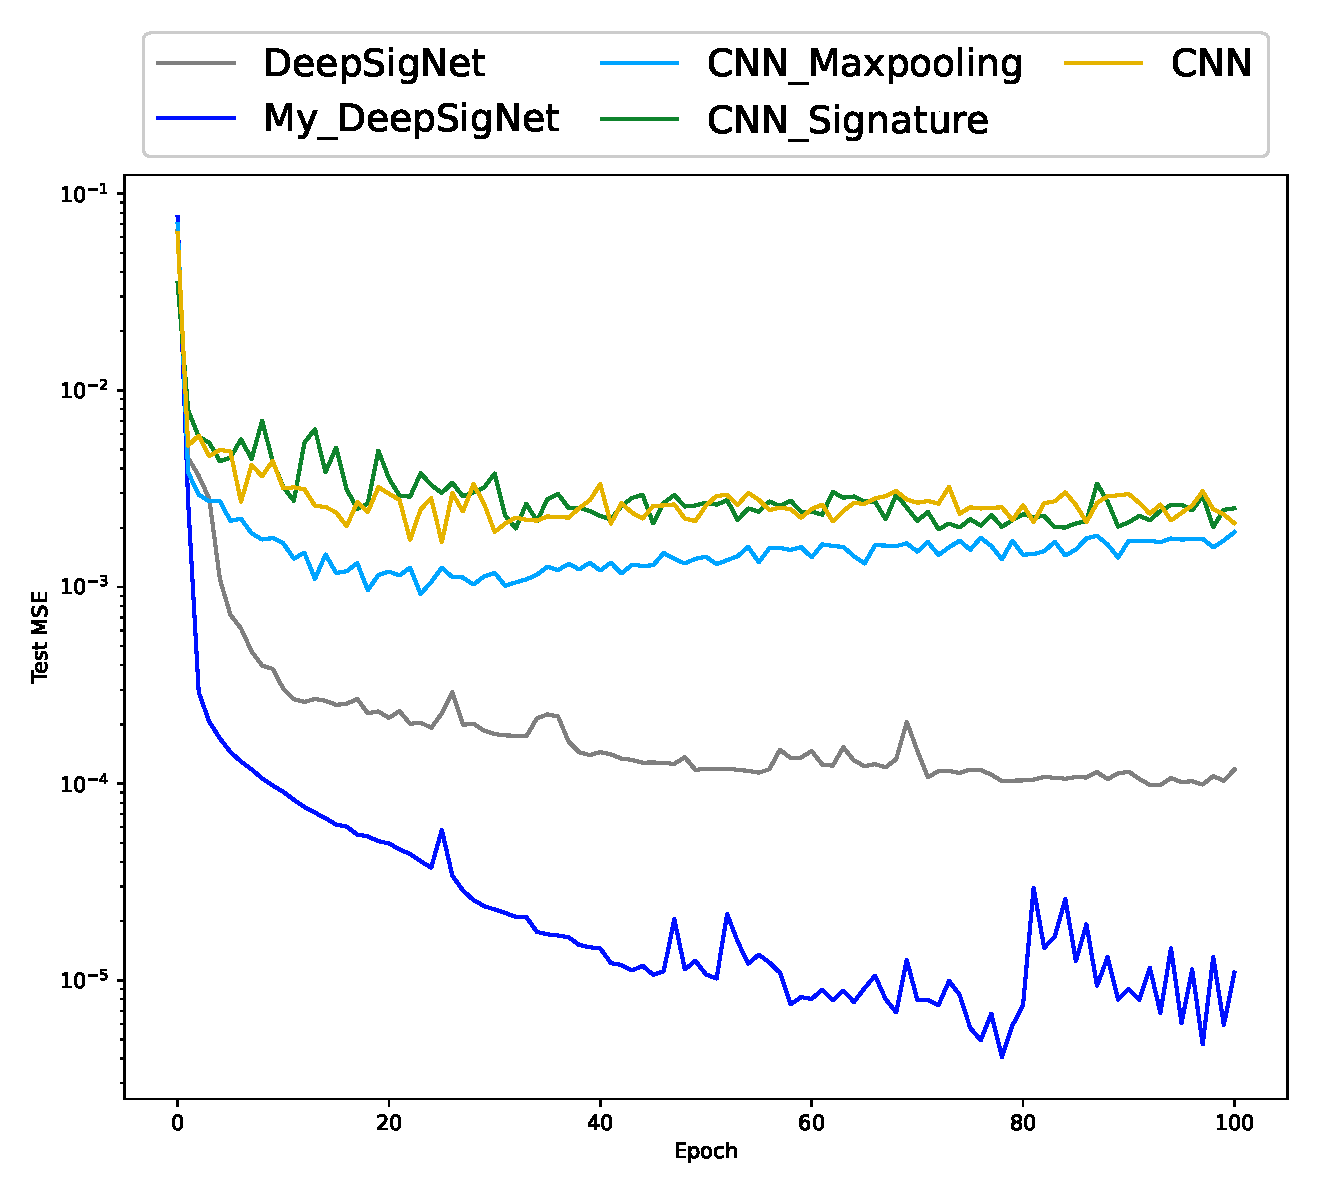
\includegraphics[width=0.32\textwidth]{fig//fBm_grid=100_Hdiscrete.eps}}
	\subfigure[$Input\,length=100$.]{
\includegraphics[width=0.32\textwidth]{fig//fBm_grid=100_Huniform.eps}}
	\subfigure[$Input\,length=100$.]{
\includegraphics[width=0.32\textwidth]{fig//fBm_grid=100_Hbeta.eps}}
	\subfigure[$Input\,length=200$.]{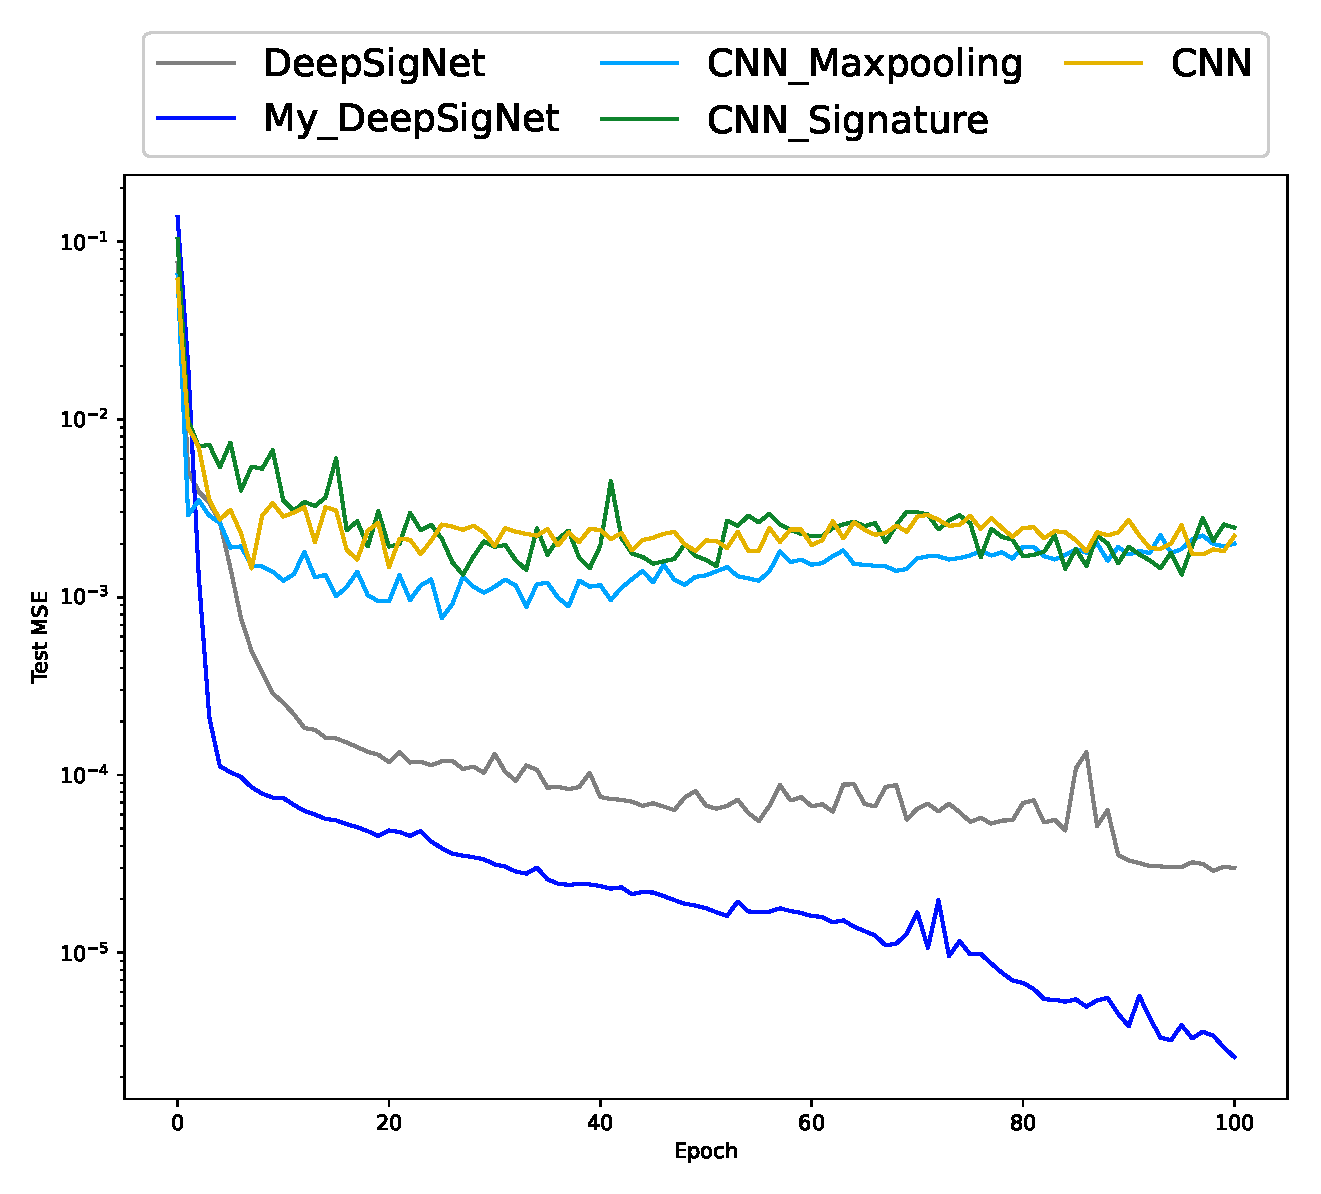
\includegraphics[width=0.32\textwidth]{fig//fBm_grid=200_Hdiscrete.eps}}
	\subfigure[$Input\,length=200$.]{
\includegraphics[width=0.32\textwidth]{fig//fBm_grid=200_Huniform.eps}}
	\subfigure[$Input\,length=200$.]{
\includegraphics[width=0.32\textwidth]{fig//fBm_grid=200_Hbeta.eps}}
	\subfigure[$Input\,length=300$.]{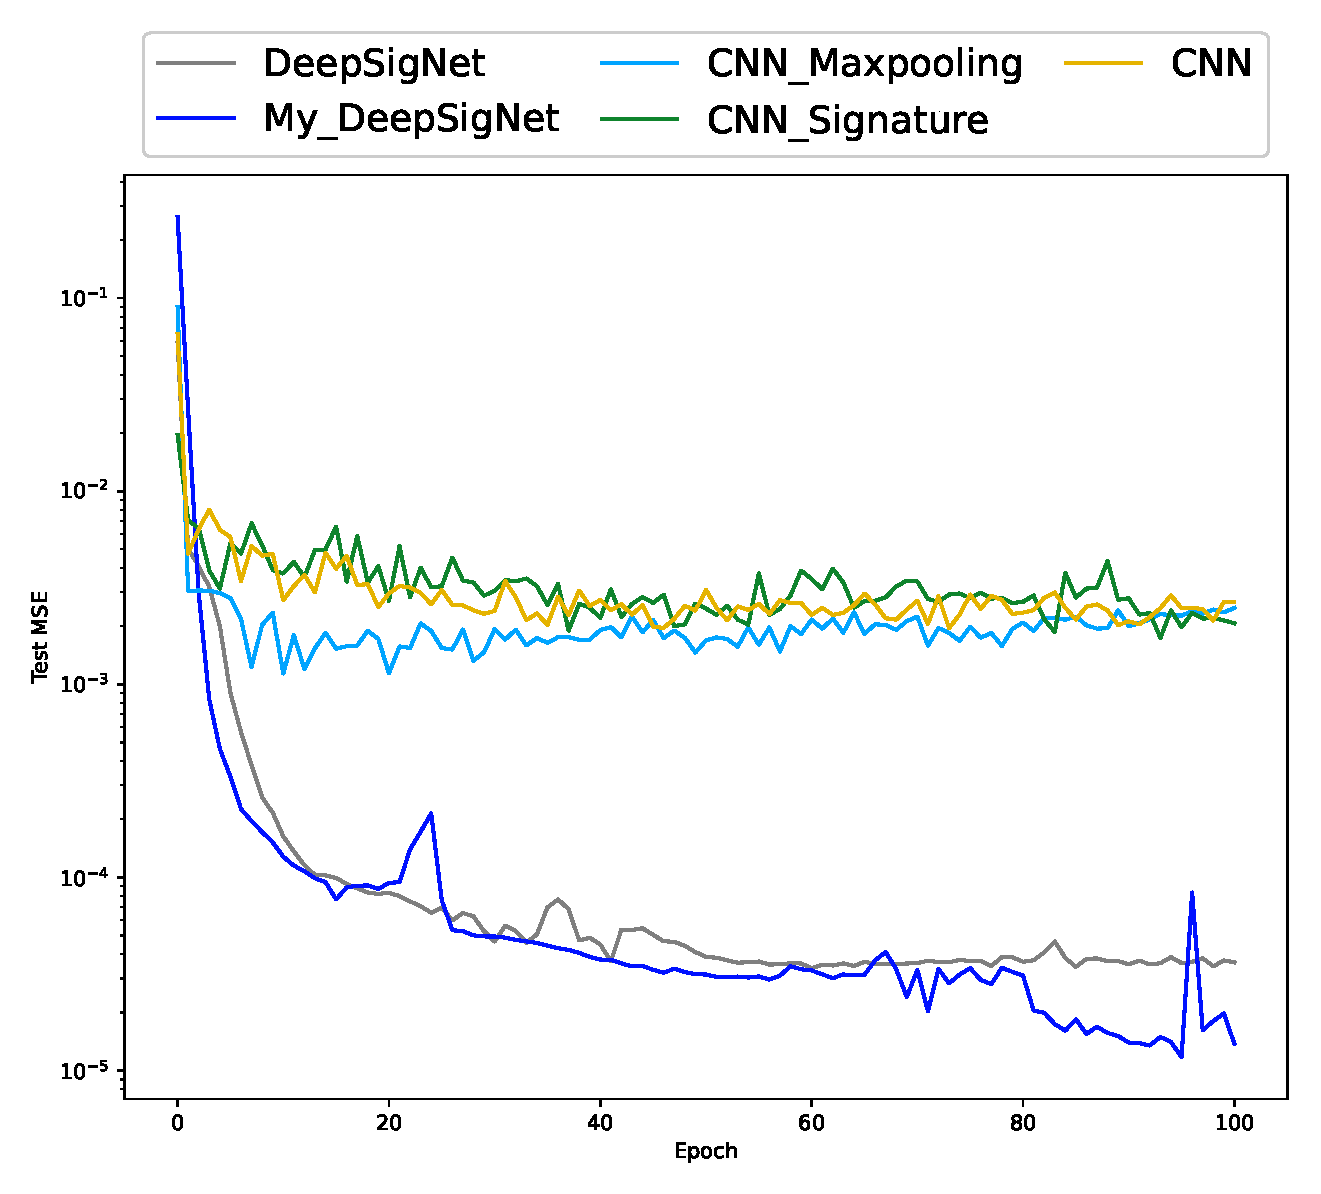
\includegraphics[width=0.32\textwidth]{fig//fBm_grid=300_Hdiscrete.eps}}
	\subfigure[$Input\,length=300$.]{
\includegraphics[width=0.32\textwidth]{fig//fBm_grid=300_Huniform.eps}}
	\subfigure[$Input\,length=300$.]{
\includegraphics[width=0.32\textwidth]{fig//fBm_grid=300_Hbeta.eps}}
	\subfigure[$Input\,length=400$.]{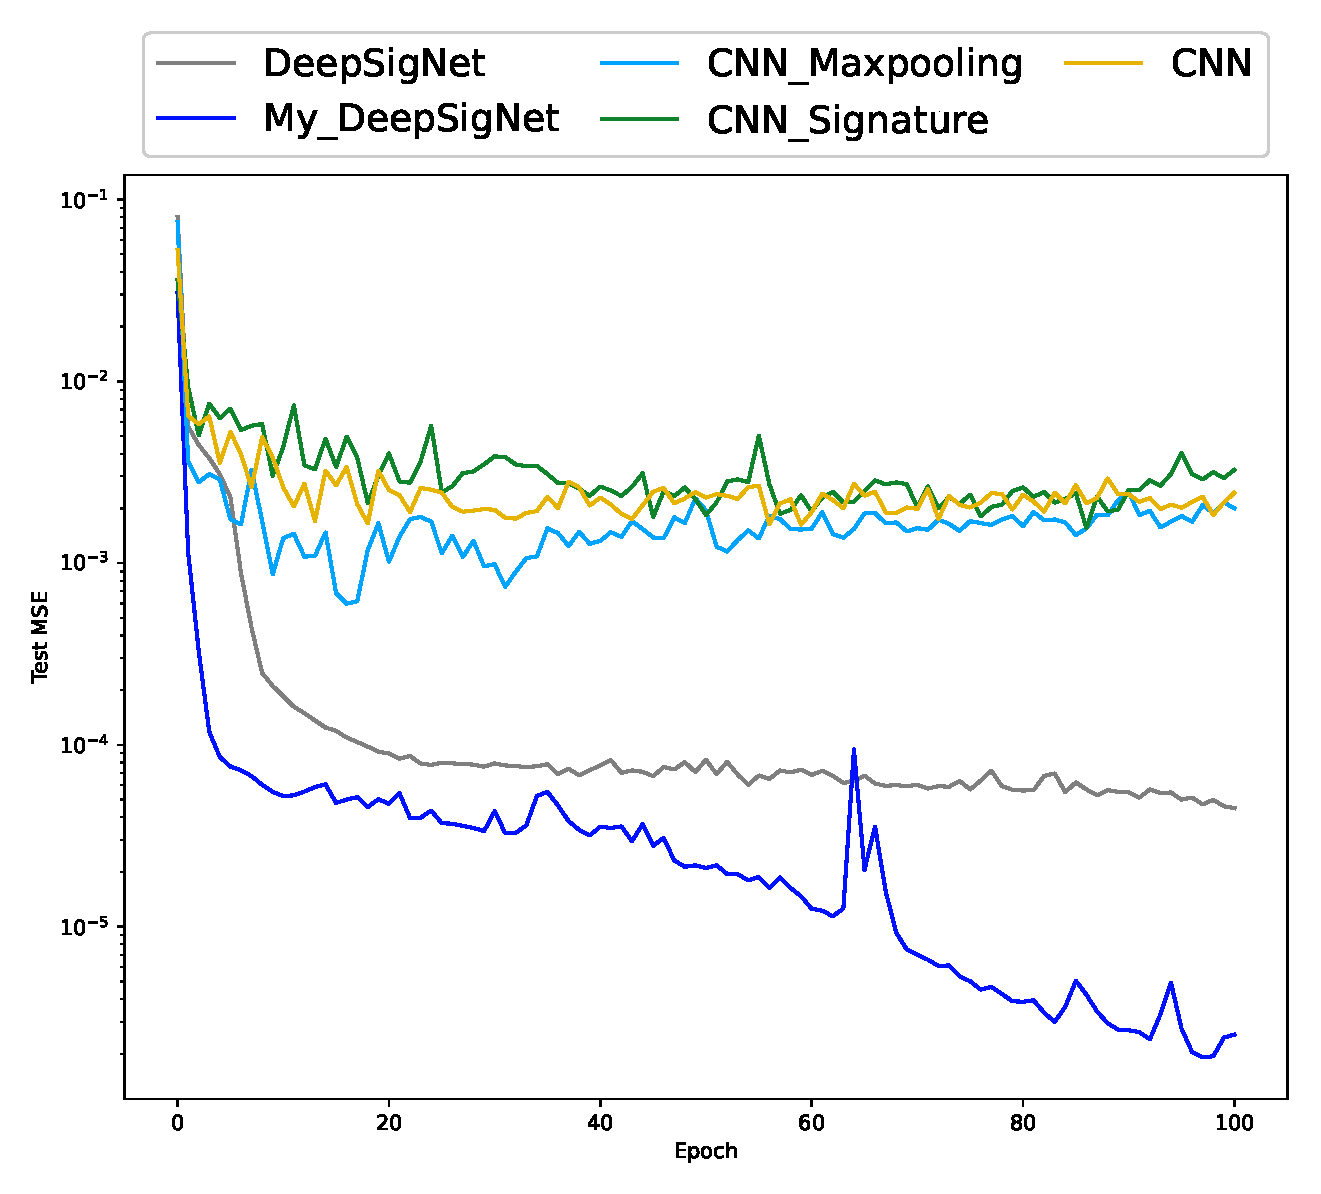
\includegraphics[width=0.32\textwidth]{fig//fBm_grid=400_Hdiscrete.eps}}
	\subfigure[$Input\,length=400$.]{
\includegraphics[width=0.32\textwidth]{fig//fBm_grid=400_Huniform.eps}}
	\subfigure[$Input\,length=400$.]{
\includegraphics[width=0.32\textwidth]{fig//fBm_grid=400_Hbeta.eps}}
	\subfigure[$Input\,length=500$.]{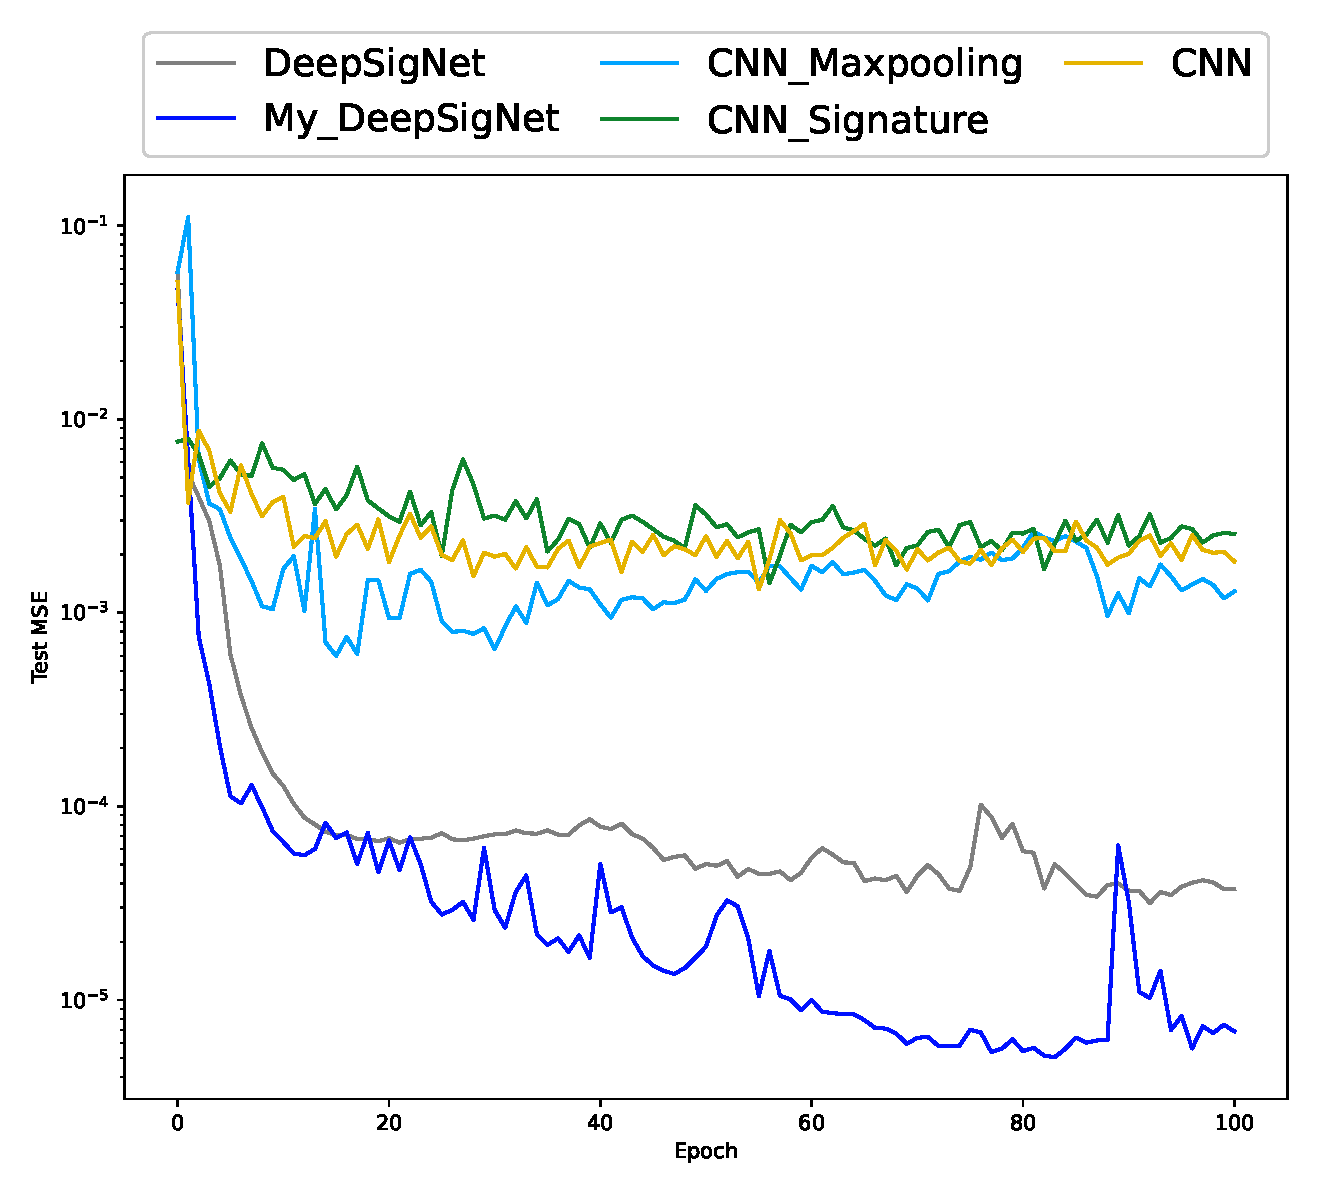
\includegraphics[width=0.32\textwidth]{fig//fBm_grid=500_Hdiscrete.eps}}
	\subfigure[$Input\,length=500$.]{
\includegraphics[width=0.32\textwidth]{fig//fBm_grid=500_Huniform.eps}}
	\subfigure[$Input\,length=500$.]{
\includegraphics[width=0.32\textwidth]{fig//fBm_grid=500_Hbeta.eps}}
	\caption{Loss plot for fractional Brownian motions with (Left:) discretised $H$; (Middle:) $H\sim\text{Uniform}(0,0.5)$; (Right:) $H\sim\text{Beta}(1,9)$. }
	\label{fig-fBm-loss}
\end{figure}

\begin{figure}[H]
	\centering
	\subfigure[$Input\,length=100$.]{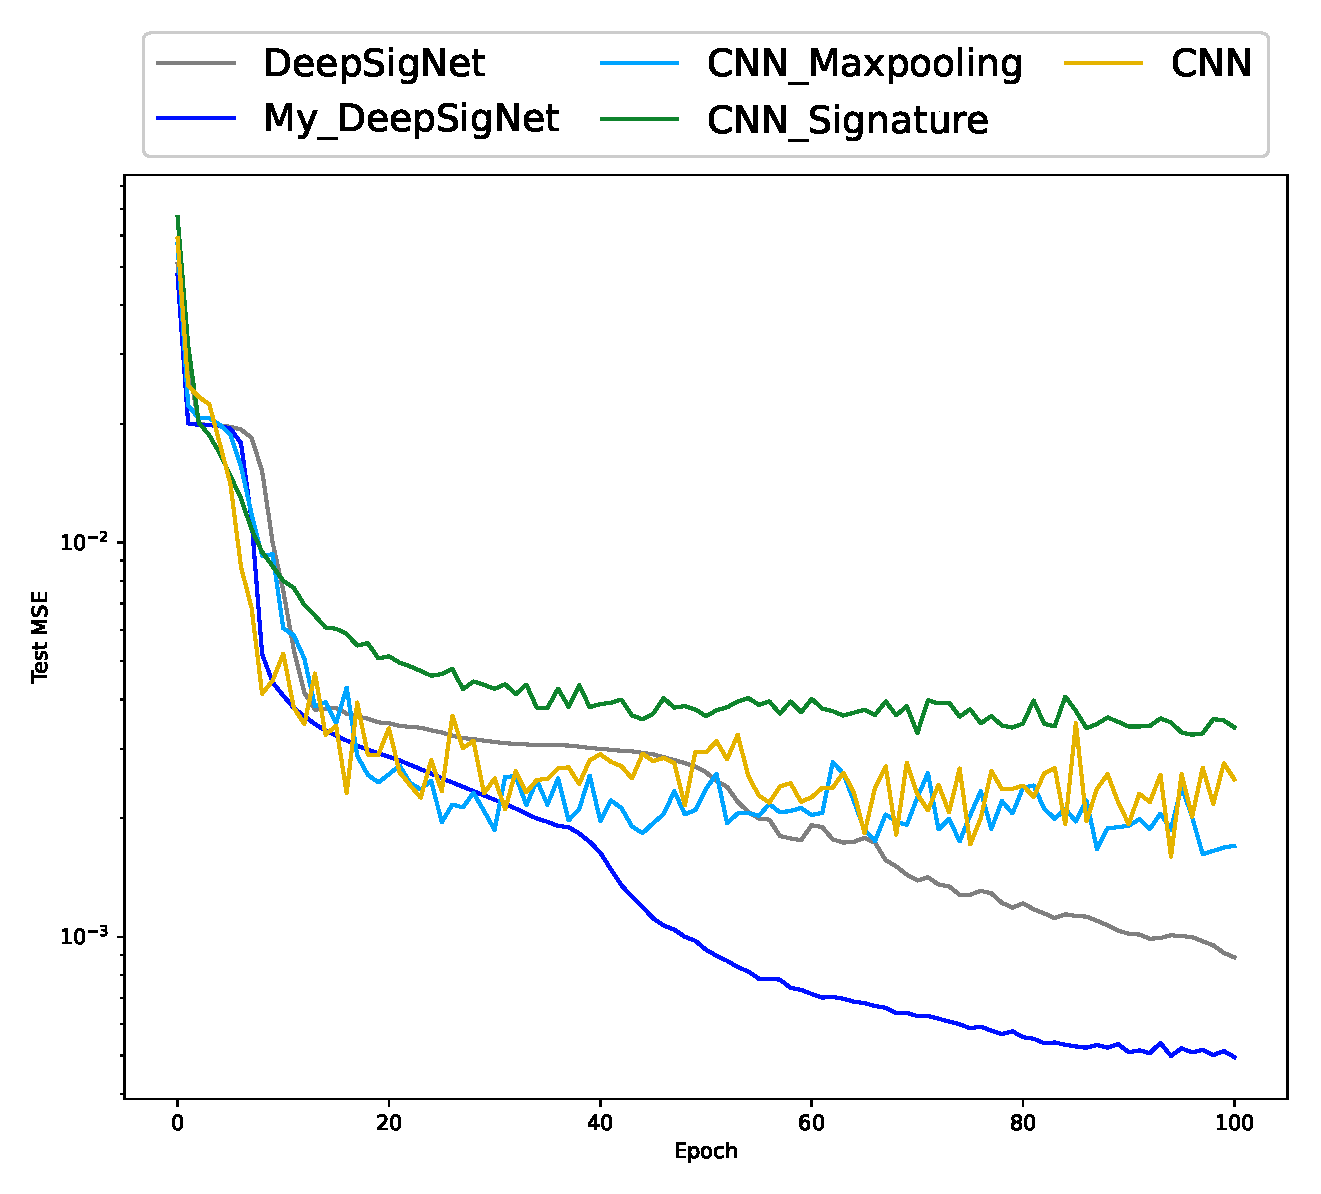
\includegraphics[width=0.32\textwidth]{fig//rBergomi_grid=100_Hdiscrete_eta=1_v0=0.01.eps}}
	\subfigure[$Input\,length=100$.]{
\includegraphics[width=0.32\textwidth]{fig//rBergomi_grid=100_Huniform_eta=1_v0=0.01.eps}}
	\subfigure[$Input\,length=100$.]{
\includegraphics[width=0.32\textwidth]{fig//rBergomi_grid=100_Hbeta_eta=1_v0=0.01.eps}}
	\subfigure[$Input\,length=200$.]{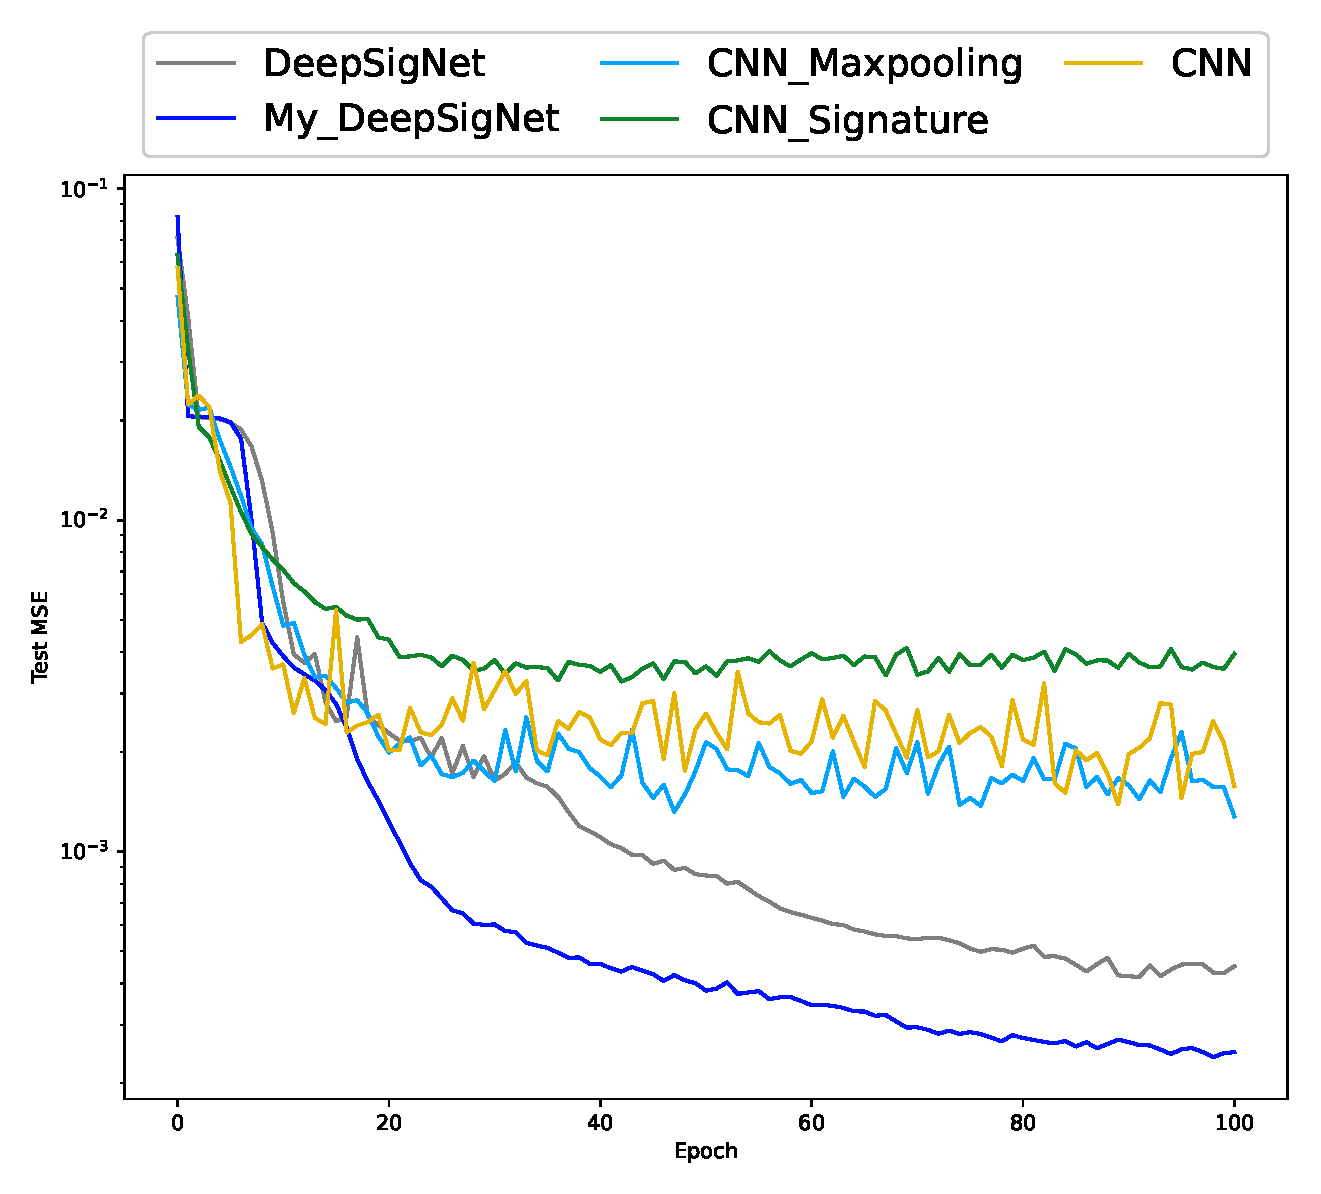
\includegraphics[width=0.32\textwidth]{fig//rBergomi_grid=200_Hdiscrete_eta=1_v0=0.01.eps}}
	\subfigure[$Input\,length=200$.]{
\includegraphics[width=0.32\textwidth]{fig//rBergomi_grid=200_Huniform_eta=1_v0=0.01.eps}}
	\subfigure[$Input\,length=200$.]{
\includegraphics[width=0.32\textwidth]{fig//rBergomi_grid=200_Hbeta_eta=1_v0=0.01.eps}}
	\subfigure[$Input\,length=300$.]{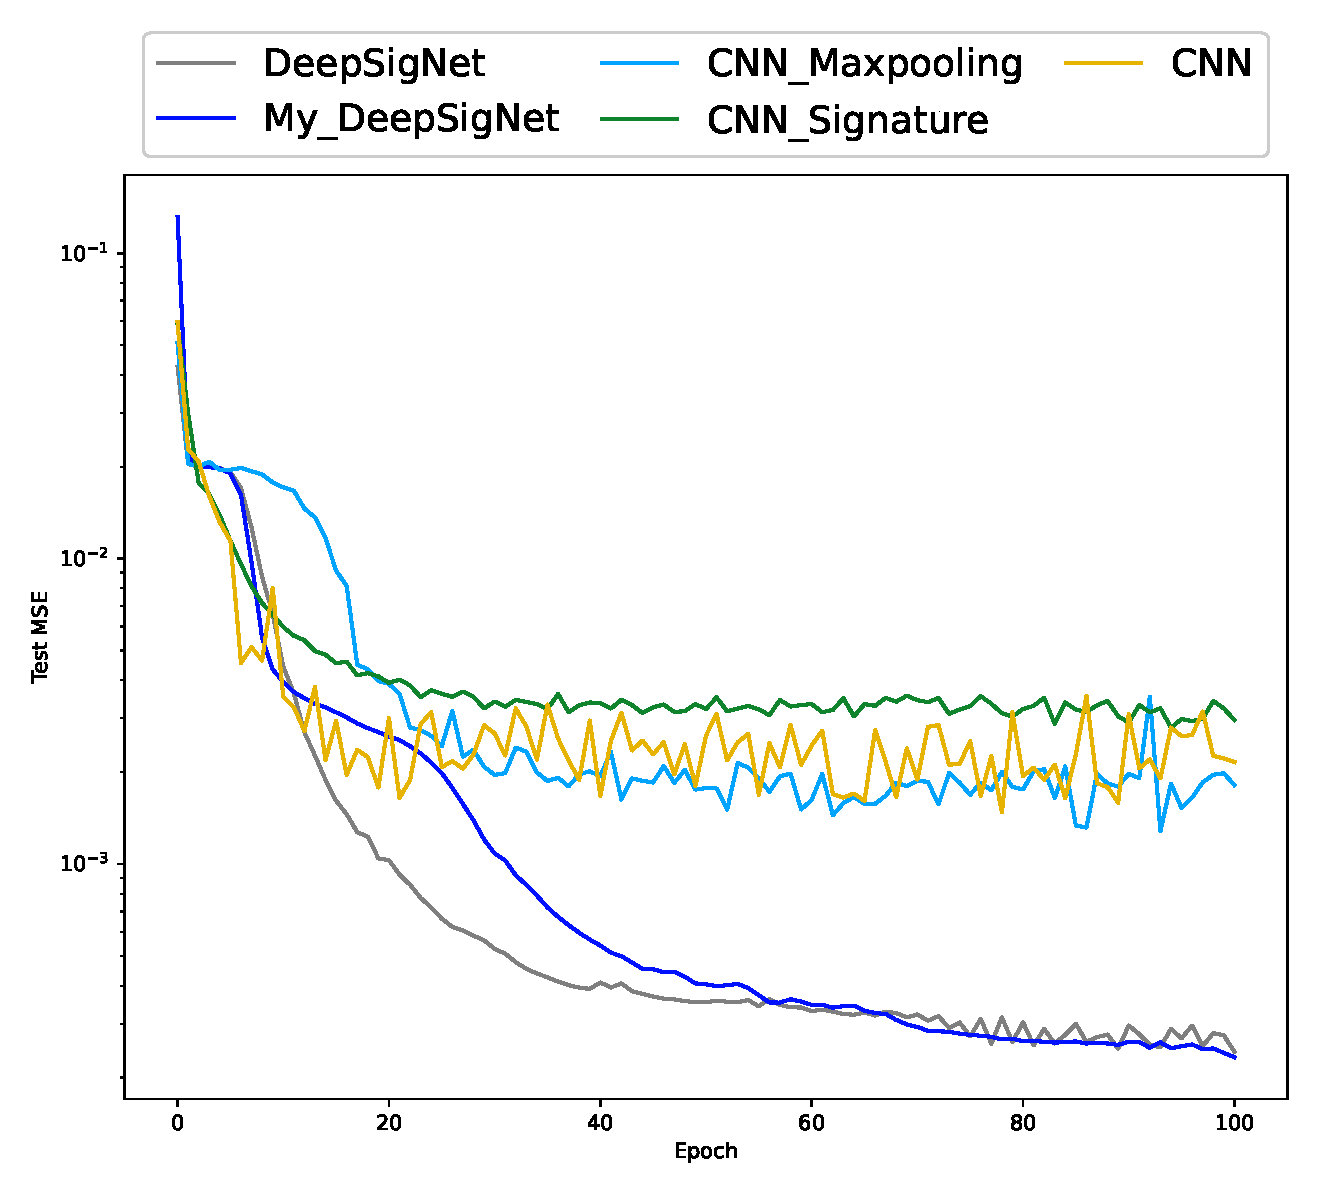
\includegraphics[width=0.32\textwidth]{fig//rBergomi_grid=300_Hdiscrete_eta=1_v0=0.01.eps}}
	\subfigure[$Input\,length=300$.]{
\includegraphics[width=0.32\textwidth]{fig//rBergomi_grid=300_Huniform_eta=1_v0=0.01.eps}}
	\subfigure[$Input\,length=300$.]{
\includegraphics[width=0.32\textwidth]{fig//rBergomi_grid=300_Hbeta_eta=1_v0=0.01.eps}}
	\subfigure[$Input\,length=400$.]{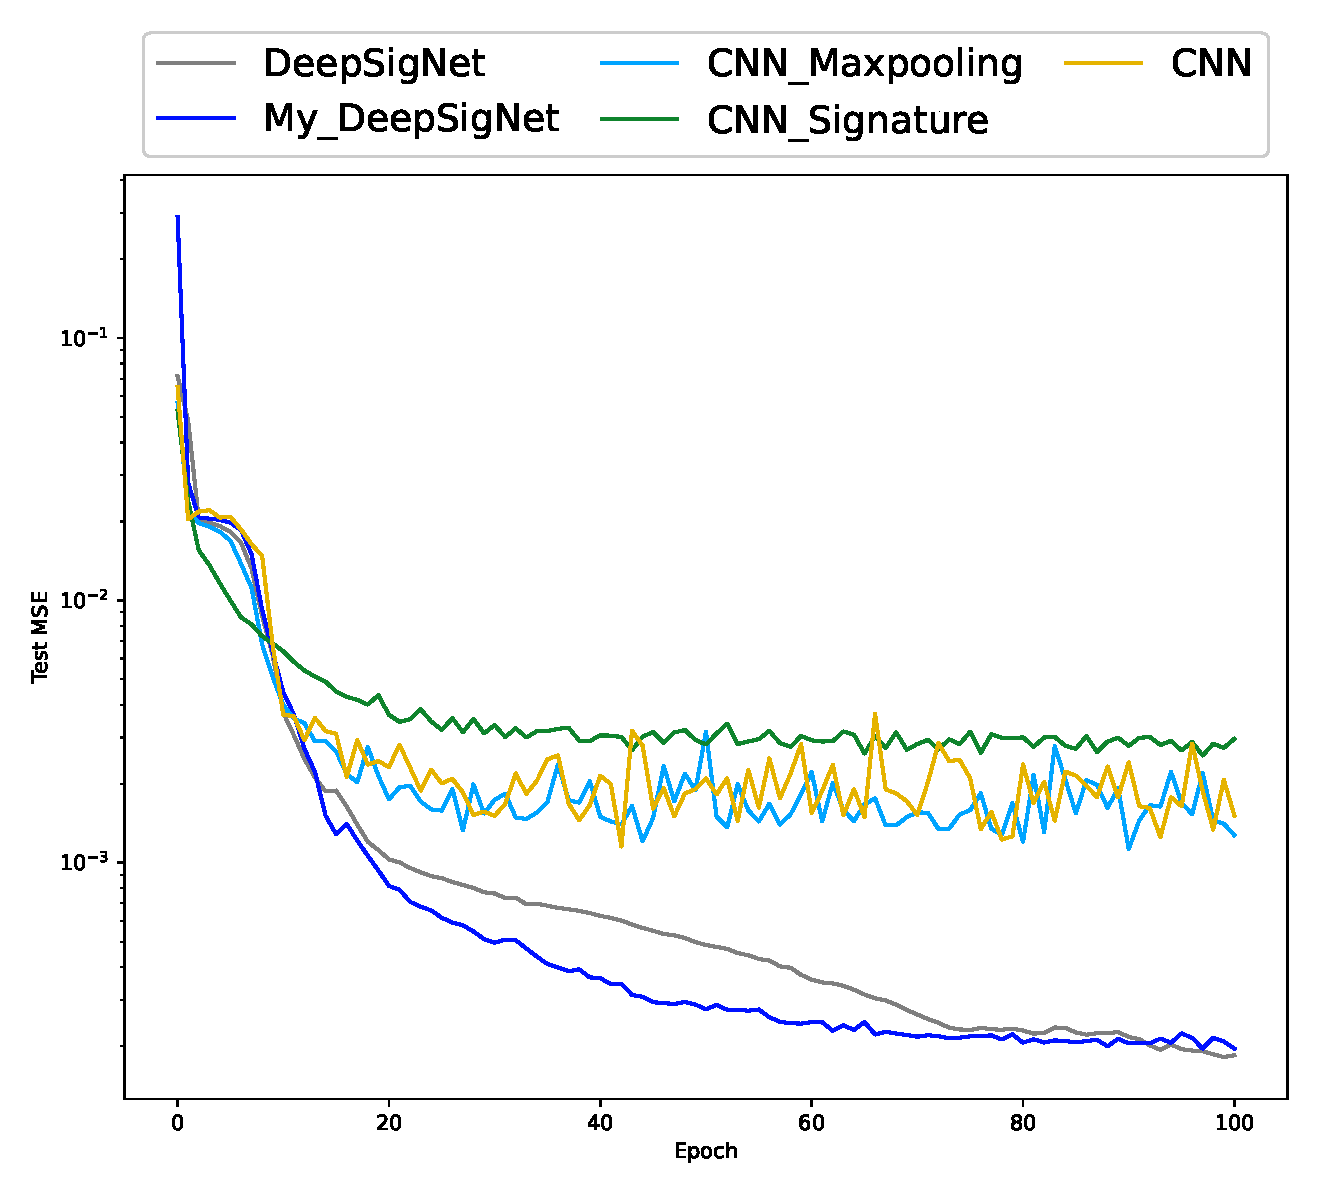
\includegraphics[width=0.32\textwidth]{fig//rBergomi_grid=400_Hdiscrete_eta=1_v0=0.01.eps}}
	\subfigure[$Input\,length=400$.]{
\includegraphics[width=0.32\textwidth]{fig//rBergomi_grid=400_Huniform_eta=1_v0=0.01.eps}}
	\subfigure[$Input\,length=400$.]{
\includegraphics[width=0.32\textwidth]{fig//rBergomi_grid=400_Hbeta_eta=1_v0=0.01.eps}}
	\subfigure[$Input\,length=500$.]{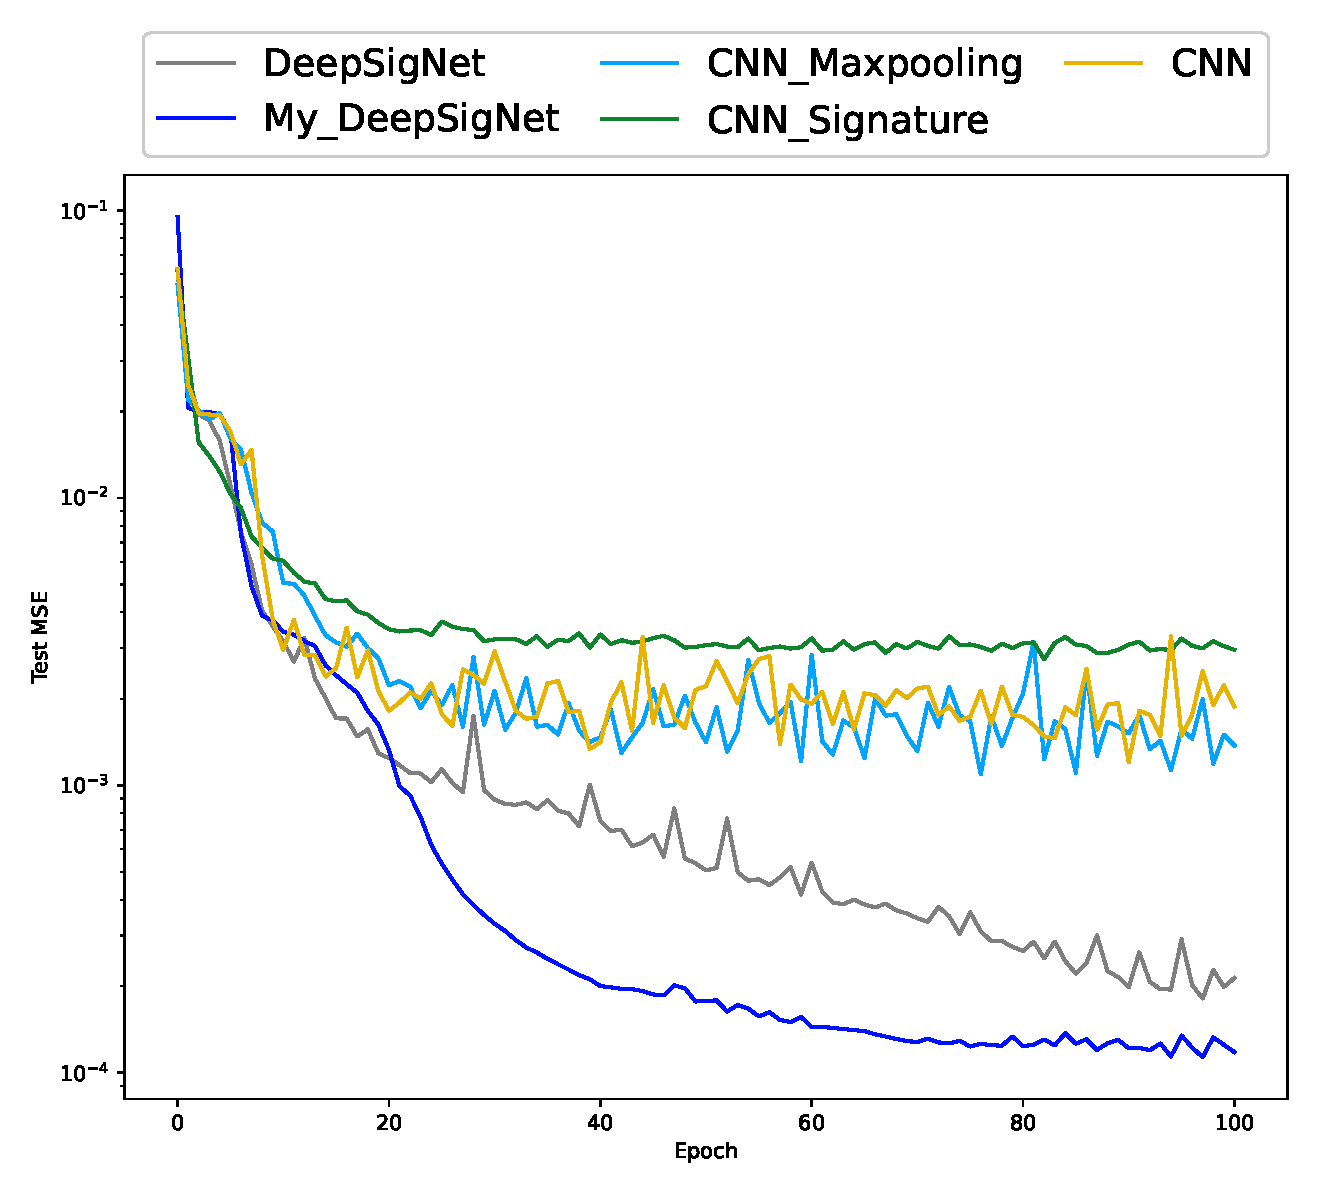
\includegraphics[width=0.32\textwidth]{fig//rBergomi_grid=500_Hdiscrete_eta=1_v0=0.01.eps}}
	\subfigure[$Input\,length=500$.]{
\includegraphics[width=0.32\textwidth]{fig//rBergomi_grid=500_Huniform_eta=1_v0=0.01.eps}}
	\subfigure[$Input\,length=500$.]{
\includegraphics[width=0.32\textwidth]{fig//rBergomi_grid=500_Hbeta_eta=1_v0=0.01.eps}}
	\caption{Loss plot for rBergomi volatility processes with (Left:) discretised $H$; (Middle:) $H\sim\text{Uniform}(0,0.5)$; (Right:) $H\sim\text{Beta}(1,9)$. }
	\label{fig-rBergomi-loss}
\end{figure}
\end{document}
